\documentclass{article}
\usepackage{iclr2027_conference,times}
\renewcommand{\ttdefault}{cmtt}
%%%%% NEW MATH DEFINITIONS %%%%%

\usepackage{amsmath,amsfonts,bm}

% Mark sections of captions for referring to divisions of figures
\newcommand{\figleft}{{\em (Left)}}
\newcommand{\figcenter}{{\em (Center)}}
\newcommand{\figright}{{\em (Right)}}
\newcommand{\figtop}{{\em (Top)}}
\newcommand{\figbottom}{{\em (Bottom)}}
\newcommand{\captiona}{{\em (a)}}
\newcommand{\captionb}{{\em (b)}}
\newcommand{\captionc}{{\em (c)}}
\newcommand{\captiond}{{\em (d)}}

% Highlight a newly defined term
\newcommand{\newterm}[1]{{\bf #1}}


% Figure reference, lower-case.
\def\figref#1{figure~\ref{#1}}
% Figure reference, capital. For start of sentence
\def\Figref#1{Figure~\ref{#1}}
\def\twofigref#1#2{figures \ref{#1} and \ref{#2}}
\def\quadfigref#1#2#3#4{figures \ref{#1}, \ref{#2}, \ref{#3} and \ref{#4}}
% Section reference, lower-case.
\def\secref#1{section~\ref{#1}}
% Section reference, capital.
\def\Secref#1{Section~\ref{#1}}
% Reference to two sections.
\def\twosecrefs#1#2{sections \ref{#1} and \ref{#2}}
% Reference to three sections.
\def\secrefs#1#2#3{sections \ref{#1}, \ref{#2} and \ref{#3}}
% Reference to an equation, lower-case.
\def\eqref#1{equation~\ref{#1}}
% Reference to an equation, upper case
\def\Eqref#1{Equation~\ref{#1}}
% A raw reference to an equation---avoid using if possible
\def\plaineqref#1{\ref{#1}}
% Reference to a chapter, lower-case.
\def\chapref#1{chapter~\ref{#1}}
% Reference to an equation, upper case.
\def\Chapref#1{Chapter~\ref{#1}}
% Reference to a range of chapters
\def\rangechapref#1#2{chapters\ref{#1}--\ref{#2}}
% Reference to an algorithm, lower-case.
\def\algref#1{algorithm~\ref{#1}}
% Reference to an algorithm, upper case.
\def\Algref#1{Algorithm~\ref{#1}}
\def\twoalgref#1#2{algorithms \ref{#1} and \ref{#2}}
\def\Twoalgref#1#2{Algorithms \ref{#1} and \ref{#2}}
% Reference to a part, lower case
\def\partref#1{part~\ref{#1}}
% Reference to a part, upper case
\def\Partref#1{Part~\ref{#1}}
\def\twopartref#1#2{parts \ref{#1} and \ref{#2}}

\def\ceil#1{\lceil #1 \rceil}
\def\floor#1{\lfloor #1 \rfloor}
\def\1{\bm{1}}
\newcommand{\train}{\mathcal{D}}
\newcommand{\valid}{\mathcal{D_{\mathrm{valid}}}}
\newcommand{\test}{\mathcal{D_{\mathrm{test}}}}

\def\eps{{\epsilon}}


% Random variables
\def\reta{{\textnormal{$\eta$}}}
\def\ra{{\textnormal{a}}}
\def\rb{{\textnormal{b}}}
\def\rc{{\textnormal{c}}}
\def\rd{{\textnormal{d}}}
\def\re{{\textnormal{e}}}
\def\rf{{\textnormal{f}}}
\def\rg{{\textnormal{g}}}
\def\rh{{\textnormal{h}}}
\def\ri{{\textnormal{i}}}
\def\rj{{\textnormal{j}}}
\def\rk{{\textnormal{k}}}
\def\rl{{\textnormal{l}}}
% rm is already a command, just don't name any random variables m
\def\rn{{\textnormal{n}}}
\def\ro{{\textnormal{o}}}
\def\rp{{\textnormal{p}}}
\def\rq{{\textnormal{q}}}
\def\rr{{\textnormal{r}}}
\def\rs{{\textnormal{s}}}
\def\rt{{\textnormal{t}}}
\def\ru{{\textnormal{u}}}
\def\rv{{\textnormal{v}}}
\def\rw{{\textnormal{w}}}
\def\rx{{\textnormal{x}}}
\def\ry{{\textnormal{y}}}
\def\rz{{\textnormal{z}}}

% Random vectors
\def\rvepsilon{{\mathbf{\epsilon}}}
\def\rvtheta{{\mathbf{\theta}}}
\def\rva{{\mathbf{a}}}
\def\rvb{{\mathbf{b}}}
\def\rvc{{\mathbf{c}}}
\def\rvd{{\mathbf{d}}}
\def\rve{{\mathbf{e}}}
\def\rvf{{\mathbf{f}}}
\def\rvg{{\mathbf{g}}}
\def\rvh{{\mathbf{h}}}
\def\rvu{{\mathbf{i}}}
\def\rvj{{\mathbf{j}}}
\def\rvk{{\mathbf{k}}}
\def\rvl{{\mathbf{l}}}
\def\rvm{{\mathbf{m}}}
\def\rvn{{\mathbf{n}}}
\def\rvo{{\mathbf{o}}}
\def\rvp{{\mathbf{p}}}
\def\rvq{{\mathbf{q}}}
\def\rvr{{\mathbf{r}}}
\def\rvs{{\mathbf{s}}}
\def\rvt{{\mathbf{t}}}
\def\rvu{{\mathbf{u}}}
\def\rvv{{\mathbf{v}}}
\def\rvw{{\mathbf{w}}}
\def\rvx{{\mathbf{x}}}
\def\rvy{{\mathbf{y}}}
\def\rvz{{\mathbf{z}}}

% Elements of random vectors
\def\erva{{\textnormal{a}}}
\def\ervb{{\textnormal{b}}}
\def\ervc{{\textnormal{c}}}
\def\ervd{{\textnormal{d}}}
\def\erve{{\textnormal{e}}}
\def\ervf{{\textnormal{f}}}
\def\ervg{{\textnormal{g}}}
\def\ervh{{\textnormal{h}}}
\def\ervi{{\textnormal{i}}}
\def\ervj{{\textnormal{j}}}
\def\ervk{{\textnormal{k}}}
\def\ervl{{\textnormal{l}}}
\def\ervm{{\textnormal{m}}}
\def\ervn{{\textnormal{n}}}
\def\ervo{{\textnormal{o}}}
\def\ervp{{\textnormal{p}}}
\def\ervq{{\textnormal{q}}}
\def\ervr{{\textnormal{r}}}
\def\ervs{{\textnormal{s}}}
\def\ervt{{\textnormal{t}}}
\def\ervu{{\textnormal{u}}}
\def\ervv{{\textnormal{v}}}
\def\ervw{{\textnormal{w}}}
\def\ervx{{\textnormal{x}}}
\def\ervy{{\textnormal{y}}}
\def\ervz{{\textnormal{z}}}

% Random matrices
\def\rmA{{\mathbf{A}}}
\def\rmB{{\mathbf{B}}}
\def\rmC{{\mathbf{C}}}
\def\rmD{{\mathbf{D}}}
\def\rmE{{\mathbf{E}}}
\def\rmF{{\mathbf{F}}}
\def\rmG{{\mathbf{G}}}
\def\rmH{{\mathbf{H}}}
\def\rmI{{\mathbf{I}}}
\def\rmJ{{\mathbf{J}}}
\def\rmK{{\mathbf{K}}}
\def\rmL{{\mathbf{L}}}
\def\rmM{{\mathbf{M}}}
\def\rmN{{\mathbf{N}}}
\def\rmO{{\mathbf{O}}}
\def\rmP{{\mathbf{P}}}
\def\rmQ{{\mathbf{Q}}}
\def\rmR{{\mathbf{R}}}
\def\rmS{{\mathbf{S}}}
\def\rmT{{\mathbf{T}}}
\def\rmU{{\mathbf{U}}}
\def\rmV{{\mathbf{V}}}
\def\rmW{{\mathbf{W}}}
\def\rmX{{\mathbf{X}}}
\def\rmY{{\mathbf{Y}}}
\def\rmZ{{\mathbf{Z}}}

% Elements of random matrices
\def\ermA{{\textnormal{A}}}
\def\ermB{{\textnormal{B}}}
\def\ermC{{\textnormal{C}}}
\def\ermD{{\textnormal{D}}}
\def\ermE{{\textnormal{E}}}
\def\ermF{{\textnormal{F}}}
\def\ermG{{\textnormal{G}}}
\def\ermH{{\textnormal{H}}}
\def\ermI{{\textnormal{I}}}
\def\ermJ{{\textnormal{J}}}
\def\ermK{{\textnormal{K}}}
\def\ermL{{\textnormal{L}}}
\def\ermM{{\textnormal{M}}}
\def\ermN{{\textnormal{N}}}
\def\ermO{{\textnormal{O}}}
\def\ermP{{\textnormal{P}}}
\def\ermQ{{\textnormal{Q}}}
\def\ermR{{\textnormal{R}}}
\def\ermS{{\textnormal{S}}}
\def\ermT{{\textnormal{T}}}
\def\ermU{{\textnormal{U}}}
\def\ermV{{\textnormal{V}}}
\def\ermW{{\textnormal{W}}}
\def\ermX{{\textnormal{X}}}
\def\ermY{{\textnormal{Y}}}
\def\ermZ{{\textnormal{Z}}}

% Vectors
\def\vzero{{\bm{0}}}
\def\vone{{\bm{1}}}
\def\vmu{{\bm{\mu}}}
\def\vtheta{{\bm{\theta}}}
\def\va{{\bm{a}}}
\def\vb{{\bm{b}}}
\def\vc{{\bm{c}}}
\def\vd{{\bm{d}}}
\def\ve{{\bm{e}}}
\def\vf{{\bm{f}}}
\def\vg{{\bm{g}}}
\def\vh{{\bm{h}}}
\def\vi{{\bm{i}}}
\def\vj{{\bm{j}}}
\def\vk{{\bm{k}}}
\def\vl{{\bm{l}}}
\def\vm{{\bm{m}}}
\def\vn{{\bm{n}}}
\def\vo{{\bm{o}}}
\def\vp{{\bm{p}}}
\def\vq{{\bm{q}}}
\def\vr{{\bm{r}}}
\def\vs{{\bm{s}}}
\def\vt{{\bm{t}}}
\def\vu{{\bm{u}}}
\def\vv{{\bm{v}}}
\def\vw{{\bm{w}}}
\def\vx{{\bm{x}}}
\def\vy{{\bm{y}}}
\def\vz{{\bm{z}}}

% Elements of vectors
\def\evalpha{{\alpha}}
\def\evbeta{{\beta}}
\def\evepsilon{{\epsilon}}
\def\evlambda{{\lambda}}
\def\evomega{{\omega}}
\def\evmu{{\mu}}
\def\evpsi{{\psi}}
\def\evsigma{{\sigma}}
\def\evtheta{{\theta}}
\def\eva{{a}}
\def\evb{{b}}
\def\evc{{c}}
\def\evd{{d}}
\def\eve{{e}}
\def\evf{{f}}
\def\evg{{g}}
\def\evh{{h}}
\def\evi{{i}}
\def\evj{{j}}
\def\evk{{k}}
\def\evl{{l}}
\def\evm{{m}}
\def\evn{{n}}
\def\evo{{o}}
\def\evp{{p}}
\def\evq{{q}}
\def\evr{{r}}
\def\evs{{s}}
\def\evt{{t}}
\def\evu{{u}}
\def\evv{{v}}
\def\evw{{w}}
\def\evx{{x}}
\def\evy{{y}}
\def\evz{{z}}

% Matrix
\def\mA{{\bm{A}}}
\def\mB{{\bm{B}}}
\def\mC{{\bm{C}}}
\def\mD{{\bm{D}}}
\def\mE{{\bm{E}}}
\def\mF{{\bm{F}}}
\def\mG{{\bm{G}}}
\def\mH{{\bm{H}}}
\def\mI{{\bm{I}}}
\def\mJ{{\bm{J}}}
\def\mK{{\bm{K}}}
\def\mL{{\bm{L}}}
\def\mM{{\bm{M}}}
\def\mN{{\bm{N}}}
\def\mO{{\bm{O}}}
\def\mP{{\bm{P}}}
\def\mQ{{\bm{Q}}}
\def\mR{{\bm{R}}}
\def\mS{{\bm{S}}}
\def\mT{{\bm{T}}}
\def\mU{{\bm{U}}}
\def\mV{{\bm{V}}}
\def\mW{{\bm{W}}}
\def\mX{{\bm{X}}}
\def\mY{{\bm{Y}}}
\def\mZ{{\bm{Z}}}
\def\mBeta{{\bm{\beta}}}
\def\mPhi{{\bm{\Phi}}}
\def\mLambda{{\bm{\Lambda}}}
\def\mSigma{{\bm{\Sigma}}}

% Tensor
\DeclareMathAlphabet{\mathsfit}{\encodingdefault}{\sfdefault}{m}{sl}
\SetMathAlphabet{\mathsfit}{bold}{\encodingdefault}{\sfdefault}{bx}{n}
\newcommand{\tens}[1]{\bm{\mathsfit{#1}}}
\def\tA{{\tens{A}}}
\def\tB{{\tens{B}}}
\def\tC{{\tens{C}}}
\def\tD{{\tens{D}}}
\def\tE{{\tens{E}}}
\def\tF{{\tens{F}}}
\def\tG{{\tens{G}}}
\def\tH{{\tens{H}}}
\def\tI{{\tens{I}}}
\def\tJ{{\tens{J}}}
\def\tK{{\tens{K}}}
\def\tL{{\tens{L}}}
\def\tM{{\tens{M}}}
\def\tN{{\tens{N}}}
\def\tO{{\tens{O}}}
\def\tP{{\tens{P}}}
\def\tQ{{\tens{Q}}}
\def\tR{{\tens{R}}}
\def\tS{{\tens{S}}}
\def\tT{{\tens{T}}}
\def\tU{{\tens{U}}}
\def\tV{{\tens{V}}}
\def\tW{{\tens{W}}}
\def\tX{{\tens{X}}}
\def\tY{{\tens{Y}}}
\def\tZ{{\tens{Z}}}


% Graph
\def\gA{{\mathcal{A}}}
\def\gB{{\mathcal{B}}}
\def\gC{{\mathcal{C}}}
\def\gD{{\mathcal{D}}}
\def\gE{{\mathcal{E}}}
\def\gF{{\mathcal{F}}}
\def\gG{{\mathcal{G}}}
\def\gH{{\mathcal{H}}}
\def\gI{{\mathcal{I}}}
\def\gJ{{\mathcal{J}}}
\def\gK{{\mathcal{K}}}
\def\gL{{\mathcal{L}}}
\def\gM{{\mathcal{M}}}
\def\gN{{\mathcal{N}}}
\def\gO{{\mathcal{O}}}
\def\gP{{\mathcal{P}}}
\def\gQ{{\mathcal{Q}}}
\def\gR{{\mathcal{R}}}
\def\gS{{\mathcal{S}}}
\def\gT{{\mathcal{T}}}
\def\gU{{\mathcal{U}}}
\def\gV{{\mathcal{V}}}
\def\gW{{\mathcal{W}}}
\def\gX{{\mathcal{X}}}
\def\gY{{\mathcal{Y}}}
\def\gZ{{\mathcal{Z}}}

% Sets
\def\sA{{\mathbb{A}}}
\def\sB{{\mathbb{B}}}
\def\sC{{\mathbb{C}}}
\def\sD{{\mathbb{D}}}
% Don't use a set called E, because this would be the same as our symbol
% for expectation.
\def\sF{{\mathbb{F}}}
\def\sG{{\mathbb{G}}}
\def\sH{{\mathbb{H}}}
\def\sI{{\mathbb{I}}}
\def\sJ{{\mathbb{J}}}
\def\sK{{\mathbb{K}}}
\def\sL{{\mathbb{L}}}
\def\sM{{\mathbb{M}}}
\def\sN{{\mathbb{N}}}
\def\sO{{\mathbb{O}}}
\def\sP{{\mathbb{P}}}
\def\sQ{{\mathbb{Q}}}
\def\sR{{\mathbb{R}}}
\def\sS{{\mathbb{S}}}
\def\sT{{\mathbb{T}}}
\def\sU{{\mathbb{U}}}
\def\sV{{\mathbb{V}}}
\def\sW{{\mathbb{W}}}
\def\sX{{\mathbb{X}}}
\def\sY{{\mathbb{Y}}}
\def\sZ{{\mathbb{Z}}}

% Entries of a matrix
\def\emLambda{{\Lambda}}
\def\emA{{A}}
\def\emB{{B}}
\def\emC{{C}}
\def\emD{{D}}
\def\emE{{E}}
\def\emF{{F}}
\def\emG{{G}}
\def\emH{{H}}
\def\emI{{I}}
\def\emJ{{J}}
\def\emK{{K}}
\def\emL{{L}}
\def\emM{{M}}
\def\emN{{N}}
\def\emO{{O}}
\def\emP{{P}}
\def\emQ{{Q}}
\def\emR{{R}}
\def\emS{{S}}
\def\emT{{T}}
\def\emU{{U}}
\def\emV{{V}}
\def\emW{{W}}
\def\emX{{X}}
\def\emY{{Y}}
\def\emZ{{Z}}
\def\emSigma{{\Sigma}}

% entries of a tensor
% Same font as tensor, without \bm wrapper
\newcommand{\etens}[1]{\mathsfit{#1}}
\def\etLambda{{\etens{\Lambda}}}
\def\etA{{\etens{A}}}
\def\etB{{\etens{B}}}
\def\etC{{\etens{C}}}
\def\etD{{\etens{D}}}
\def\etE{{\etens{E}}}
\def\etF{{\etens{F}}}
\def\etG{{\etens{G}}}
\def\etH{{\etens{H}}}
\def\etI{{\etens{I}}}
\def\etJ{{\etens{J}}}
\def\etK{{\etens{K}}}
\def\etL{{\etens{L}}}
\def\etM{{\etens{M}}}
\def\etN{{\etens{N}}}
\def\etO{{\etens{O}}}
\def\etP{{\etens{P}}}
\def\etQ{{\etens{Q}}}
\def\etR{{\etens{R}}}
\def\etS{{\etens{S}}}
\def\etT{{\etens{T}}}
\def\etU{{\etens{U}}}
\def\etV{{\etens{V}}}
\def\etW{{\etens{W}}}
\def\etX{{\etens{X}}}
\def\etY{{\etens{Y}}}
\def\etZ{{\etens{Z}}}

% The true underlying data generating distribution
\newcommand{\pdata}{p_{\rm{data}}}
% The empirical distribution defined by the training set
\newcommand{\ptrain}{\hat{p}_{\rm{data}}}
\newcommand{\Ptrain}{\hat{P}_{\rm{data}}}
% The model distribution
\newcommand{\pmodel}{p_{\rm{model}}}
\newcommand{\Pmodel}{P_{\rm{model}}}
\newcommand{\ptildemodel}{\tilde{p}_{\rm{model}}}
% Stochastic autoencoder distributions
\newcommand{\pencode}{p_{\rm{encoder}}}
\newcommand{\pdecode}{p_{\rm{decoder}}}
\newcommand{\precons}{p_{\rm{reconstruct}}}

\newcommand{\laplace}{\mathrm{Laplace}} % Laplace distribution

\newcommand{\E}{\mathbb{E}}
\newcommand{\Ls}{\mathcal{L}}
\newcommand{\R}{\mathbb{R}}
\newcommand{\emp}{\tilde{p}}
\newcommand{\lr}{\alpha}
\newcommand{\reg}{\lambda}
\newcommand{\rect}{\mathrm{rectifier}}
\newcommand{\softmax}{\mathrm{softmax}}
\newcommand{\sigmoid}{\sigma}
\newcommand{\softplus}{\zeta}
\newcommand{\KL}{D_{\mathrm{KL}}}
\newcommand{\Var}{\mathrm{Var}}
\newcommand{\standarderror}{\mathrm{SE}}
\newcommand{\Cov}{\mathrm{Cov}}
% Wolfram Mathworld says $L^2$ is for function spaces and $\ell^2$ is for vectors
% But then they seem to use $L^2$ for vectors throughout the site, and so does
% wikipedia.
\newcommand{\normlzero}{L^0}
\newcommand{\normlone}{L^1}
\newcommand{\normltwo}{L^2}
\newcommand{\normlp}{L^p}
\newcommand{\normmax}{L^\infty}

\newcommand{\parents}{Pa} % See usage in notation.tex. Chosen to match Daphne's book.

\DeclareMathOperator*{\argmax}{arg\,max}
\DeclareMathOperator*{\argmin}{arg\,min}

\DeclareMathOperator{\sign}{sign}
\DeclareMathOperator{\Tr}{Tr}
\let\ab\allowbreak


\usepackage{hyperref}
\usepackage{url}
\usepackage{booktabs}
\usepackage{tabularx}
\usepackage{array}
\usepackage{graphicx}
\usepackage{float}
\usepackage{subcaption}
\usepackage{amsmath,amssymb,amsfonts,amsthm}
\usepackage{bm}
\usepackage{xcolor}
\usepackage{listings}

\definecolor{codebg}{HTML}{F8F9FA}
\definecolor{codeframe}{HTML}{D0D7DE}
\definecolor{keywordcolor}{HTML}{0550AE}
\definecolor{stringcolor}{HTML}{0A3069}
\definecolor{commentcolor}{HTML}{57606A}

\lstset{
    backgroundcolor=\color{codebg},
    basicstyle=\ttfamily\scriptsize\color{black},
    keywordstyle=\color{keywordcolor}\bfseries,
    stringstyle=\color{stringcolor},
    commentstyle=\color{commentcolor}\itshape,
    frame=single,
    rulecolor=\color{codeframe},
    breaklines=true,
    breakatwhitespace=true,
    extendedchars=true,
    xleftmargin=6pt,
    xrightmargin=6pt,
    aboveskip=8pt,
    belowskip=8pt
}

\hypersetup{
    colorlinks=true,
    linkcolor=blue!70!black,
    citecolor=blue!70!black,
    urlcolor=blue!70!black
}

% Metadata for decay_linear_attention
\title{\textbf{DecayLinearAttention: O(1)-Memory Linear Attention with Data-Dependent Exponential Decay}}

\author{
  \textbf{Taha Majs}\thanks{Corresponding author: tahamajs@uni.edu} \quad \textbf{Research Team} \\
  Department of Computer Science \\
  Advanced Machine Learning \& Efficiency Laboratory
}

\date{\today}


\newcommand{\fix}{\marginpar{FIX}}
\newcommand{\new}{\marginpar{NEW}}

\begin{document}

\maketitle

\begin{abstract}
Linear attention replaces the quadratic softmax with an associative kernel, 
achieving $\mathcal{O}(L)$ complexity. However, two practical issues remain: 
(i) standard linear attention has \textbf{no position-dependent decay}, so all 
past keys contribute equally to the current context, and (ii) causal 
implementations often materialize an $\mathcal{O}(L)$ intermediate state, 
negating the memory benefit.

We introduce \textbf{DecayLinearAttention}, which addresses both via:

\begin{enumerate}
\item \textbf{Data-dependent exponential decay per head.} We learn a per-head decay
  rate $\lambda_{h,t} \in (0, 1)$ from the input:
  
  $$
  \lambda\_{h,t} = \sigma\!\left(W\_g x\_t + b\_g + \ell\_h\right)
  $$
  
  where $\ell_h \in [-0.5, 0.0]$ is a per-head
  learned bias. Different heads learn different context horizons.
\item \textbf{Chunked scan with O(1) state.} We partition the sequence into chunks
  of size $C = 32$ and carry a compact state
  $S \in \mathbb{R}^{d \times d}$ between chunks. The intermediate state is
  \textbf{$\mathcal{O}(1)$ in sequence length}, in contrast to the
  $\mathcal{O}(L)$ intermediates used by cumsum-based causal linear
  attention.
\item \textbf{ELU+1 feature map.} We use $\phi(x) = \text{elu}(x) + 1$, which is
  positive and cheap.

\end{enumerate}
We support \textbf{bidirectional} attention for encoders (forward and backward 
scans averaged) and \textbf{causal} for decoders, along with GQA, RoPE, and 
\textbf{cross-attention}.

On SST-2, DecayLinearAttention achieves \textbf{50.92\%} on DistilBERT 
(baseline 90.71\%), \textbf{50.92\%} on RoBERTa (baseline 78.56\%), 
and \textbf{63.19\%} on GPT-2 (baseline 79.36\%). Peak inference VRAM is 
\textbf{347 MB MB} on DistilBERT (baseline 183 MB), and the state 
memory is \textbf{constant} in $L$.

\textbf{Keywords:} linear attention, data-dependent decay, chunked scan, O(1) 
memory, cross-attention



\vspace{0.5em}
\noindent\textbf{Keywords:} linear attention, data-dependent decay, chunked scan, O(1)
\end{abstract}

\section{01 Intro}

Draft content for decay_linear_attention.

\section{02 Related}

Draft content for decay_linear_attention.

\section{Background}

\subsection{Linear Attention}

Given $Q, K, V \in \mathbb{R}^{B \times H \times L \times d_h}$, linear 
attention computes:

\begin{equation}
O_t = \frac{\phi(q_t)^\top S_t}{\phi(q_t)^\top z_t}
\end{equation}

where:

\begin{equation}
S_t = \sum_{j \leq t} \phi(k_j) v_j^\top, \quad
z_t = \sum_{j \leq t} \phi(k_j)
\end{equation}

$S_t \in \mathbb{R}^{F \times d_h}$ and $z_t \in \mathbb{R}^F$ are the 
running state and normalizer.

\subsection{Exponential Decay Recurrence}

We add a per-token, per-head decay $\lambda_t \in (0, 1)$:

\begin{equation}
S_t = \lambda_t S_{t-1} + \phi(k_t) v_t^\top
\end{equation}

\begin{equation}
z_t = \lambda_t z_{t-1} + \phi(k_t)
\end{equation}

Unrolled:

\begin{equation}
S_t = \sum_{j \leq t} \left( \prod_{i=j+1}^{t} \lambda_i \right) \phi(k_j) v_j^\top
\end{equation}

The coefficient of contribution from position $j$ to position $t$ is:

\begin{equation}
D_{t, j} = \prod_{i=j+1}^{t} \lambda_i = \exp\!\left(\sum_{i=j+1}^{t} \log \lambda_i\right)
\end{equation}

This is an \textbf{exponential decay} with rate controlled by $\lambda$.

\subsection{Chunked Scan Algorithm}

For a chunk of $C$ tokens, we carry state $S_\text{prev}$ from the previous 
chunk. The output within the chunk is a combination of:

\begin{itemize}
\item \textbf{Intra-chunk contributions:} dense causal attention within the chunk.
\item \textbf{Inter-chunk contributions:} attention to the state $S_\text{prev}$.

\end{itemize}
The intra-chunk scores are:

\begin{equation}
\text{scores}_{ij}^\text{intra} = q_i^\top k_j \cdot 
\exp\!\left(\sum_{p=j+1}^{i} \log \lambda_p\right), \quad j \leq i
\end{equation}

The inter-chunk scores:

\begin{equation}
\text{scores}_{i}^\text{inter} = q_i^\top S_\text{prev} \cdot 
\exp\!\left(\sum_{p=1}^{i} \log \lambda_p\right)
\end{equation}

Then $S_\text{new}$ is computed by decaying $S_\text{prev}$ by the total 
chunk decay and adding the intra-chunk contributions.

\subsection{ELU+1 Feature Map}

\begin{equation}
\phi(x) = \text{elu}(x) + 1 = \begin{cases}
x + 1 & \text{if } x > 0 \\
e^x & \text{if } x \leq 0
\end{cases}
\end{equation}

\textbf{Property.} $\phi(x) > 0$ for all $x$, which ensures $z_t > 0$ and the 
normalizer is well-behaved.

\subsection{Data-Dependent Decay}

We learn $\lambda_{h,t}$ from the input:

\begin{equation}
\lambda_{h,t} = \sigma(W_g x_t + b_g + \ell_h)
\end{equation}

where:

\begin{itemize}
\item $W_g \in \mathbb{R}^{H \times d}$, $b_g \in \mathbb{R}^H$ -- learned gate.
\item $\ell_h \in \mathbb{R}$ -- per-head bias, initialized to linearly spaced
  values.

\end{itemize}
\textbf{Initialization.} $W_g = 0$, $b_g = 0$, $\ell_h = \text{linspace}(-0.5, 0.0, H)$.

\textbf{Effect.} At step 0, $\lambda_{h,t} = \sigma(\ell_h)$ -- constant per head, 
giving each head a fixed "default horizon".

\subsection{Bidirectional Attention}

For encoders, we run both forward and backward scans:

\begin{equation}
O_t = \frac{1}{2} \left( O_t^\text{fwd} + O_t^\text{bwd} \right)
\end{equation}

Each $O_t^\text{fwd}$, $O_t^\text{bwd}$ uses the same recurrence but in 
opposite directions.

\subsection{Grouped-Query Attention (GQA)}

For GQA, we expand KV heads before the scan:

\begin{equation}
K, V \in \mathbb{R}^{B \times H_{kv} \times L \times d_h}, \quad
K_\text{expanded} = \text{repeat\_kv}(K, H / H_{kv})
\end{equation}

\subsection{Notation}

\begin{table}[H]
\centering
\small
\begin{tabular}{ll}
\toprule
\textbf{Symbol} & \textbf{Meaning} \\
\midrule
$\lambda_{h,t}$ & Decay at position $t$, head $h$ \\
$\ell_h$ & Per-head bias \\
$W_g, b_g$ & Gate parameters \\
$S, z$ & Running state \\
$\phi$ & ELU+1 feature map \\
$C$ & Chunk size \\
\bottomrule
\end{tabular}
\end{table}


\section{Method}

\subsection{Overview}

DecayLinearAttention replaces standard attention with a **chunked, 
data-dependent linear recurrence**. For each head, we learn a per-token decay 
$\lambda_{h,t}$ and propagate a running state:

\[
S_t = \lambda_{h,t} S_{t-1} + \phi(k_t) v_t^\top
\tag{4.1}
\]

\[
z_t = \lambda_{h,t} z_{t-1} + \phi(k_t)
\tag{4.2}
\]

The output:

\[
O_t = \frac{\phi(q_t)^\top S_t}{\phi(q_t)^\top z_t + \epsilon}
\tag{4.3}
\]

\textbf{Figure 4.1} shows the pipeline.

\begin{lstlisting}
    X $\in$ R^{B$\times$L$\times$d}
         |
    +----+----+----+
                    
    W_q W_k W_v  decay_gate
    |   |   |    |
                  
    Q   K   V   $\lambda$_t
    |   |   |    |
                 |
     (Q)  (K) V  |
    |   |   |    |
    +---+---+----+
             
    Chunked Scan (S, z)
        |
         
    O =  (Q) S / ( (Q) z)
        |
         
    W_o
        |
         
    Output Y
\end{lstlisting}

\subsection{Data-Dependent Decay}

For each head $h$ and token $t$:

\[
\tilde{\lambda}_{h,t} = W_g x_t + b_g
\tag{4.4}
\]

\[
\lambda_{h,t} = \sigma\!\left(\tilde{\lambda}_{h,t} + \ell_h\right)
\tag{4.5}
\]

where $\ell_h$ is a \textbf{learned scalar} per head.

\textbf{Initialization.}
\begin{itemize}
\item $W_g = 0$ (no input dependence initially).
\item $b_g = 0$.
\item $\ell_h$ is initialized to linearly spaced values in
  $[{{LOG_DECAY_MIN}}, {{LOG_DECAY_MAX}}]$:

\end{itemize}
\begin{lstlisting}
  self.log_decay = nn.Parameter(torch.linspace(-0.5, 0.0, num_heads))
\end{lstlisting}

\textbf{Result.} At step 0, different heads start with different horizons:
\begin{itemize}
\item Head 0: $\lambda \approx \sigma({{LOG_DECAY_MIN}}) \approx {{LAMBDA_MIN}}$
\item Head $H-1$: $\lambda \approx \sigma({{LOG_DECAY_MAX}}) \approx {{LAMBDA_MAX}}$

\end{itemize}
This head diversity is analogous to multi-scale temporal receptive fields in 
convolutional networks.

\subsection{ELU+1 Feature Map}

\[
\phi(x) = \text{elu}(x) + 1
\tag{4.6}
\]

Applied element-wise to Q, K.

\textbf{Why ELU+1?}
\begin{itemize}
\item \textbf{Positive:} Ensures $z_t > 0$.
\item \textbf{Cheap:} No exponential or trigonometric functions.
\item \textbf{Established:} Used by Linear Transformer (Katharopoulos et al., 2020).

\end{itemize}
\subsection{Chunked Scan}

For a chunk of size $C$ starting at position $s$:

\subsubsection{Cumulative Log-Decay}

Within the chunk, we compute:

\[
\Lambda_i = \sum_{p=s}^{s+i} \log \lambda_{h,p}, \quad i \in [0, C)
\tag{4.7}
\]

via \texttt{torch.cumsum}.

\subsubsection{Intra-Chunk Attention}

For positions $i, j$ in the chunk with $j \leq i$:

\[
D_{i, j}^\text{intra} = \exp(\Lambda_i - \Lambda_j)
\tag{4.8}
\]

\[
A_{i, j}^\text{intra} = \phi(q_i)^\top \phi(k_j) \cdot D_{i, j}^\text{intra}
\tag{4.9}
\]

with $A_{i, j}^\text{intra} = 0$ for $j > i$ (causality).

Output (numerator):

\[
\text{num}_i^\text{intra} = \sum_{j \leq i} A_{i, j}^\text{intra} \cdot v_j
\tag{4.10}
\]

Normalizer (denominator):

\[
\text{denom}_i^\text{intra} = \sum_{j \leq i} A_{i, j}^\text{intra}
\tag{4.11}
\]

\subsubsection{Inter-Chunk Contribution}

Let $S_\text{prev}$, $z_\text{prev}$ be the state before the chunk. Define:

\[
D_i^\text{inter} = \exp(\Lambda_i)
\tag{4.12}
\]

Then:

\[
\text{num}_i^\text{inter} = \phi(q_i)^\top S_\text{prev} \cdot D_i^\text{inter}
\tag{4.13}
\]

\[
\text{denom}_i^\text{inter} = \phi(q_i)^\top z_\text{prev} \cdot D_i^\text{inter}
\tag{4.14}
\]

\subsubsection{Output}

\[
O_i = \frac{\text{num}_i^\text{intra} + \text{num}_i^\text{inter}}{\text{denom}_i^\text{intra} + \text{denom}_i^\text{inter} + \epsilon}
\tag{4.15}
\]

\subsubsection{State Update}

After the chunk, the state is updated for the next chunk:

\[
S_\text{new} = \exp(\Lambda_C) S_\text{prev} + \sum_{i=0}^{C-1} \exp(\Lambda_C - \Lambda_i) \phi(k_i) v_i^\top
\tag{4.16}
\]

\[
z_\text{new} = \exp(\Lambda_C) z_\text{prev} + \sum_{i=0}^{C-1} \exp(\Lambda_C - \Lambda_i) \phi(k_i)
\tag{4.17}
\]

where $\Lambda_C$ is the cumulative log-decay at the end of the chunk.

\subsection{Bidirectional Mode}

For encoders, we run the chunked scan twice:

\[
O^\text{fwd} = \text{Scan}(Q, K, V, \lambda) \quad \text{(left to right)}
\]

\[
O^\text{bwd} = \text{Scan}(Q, K, V, \lambda) \quad \text{(right to left)}
\]

where the backward scan flips the sequence, runs the forward scan, then 
flips back.

Final output:

\[
O = \frac{1}{2} (O^\text{fwd} + O^\text{bwd})
\tag{4.18}
\]

\subsection{Algorithm}

\textbf{Algorithm 1:} Chunked decay scan
\begin{lstlisting}
Input:  Q, K, V $\in$ R^{B$\times$H$\times$L$\times$d}, $\lambda$ $\in$ R^{B$\times$H$\times$L}
        chunk_size C = 32
Output: O $\in$ R^{B$\times$H$\times$L$\times$d}

 1: log_$\lambda$ $\leftarrow$ log(clamp($\lambda$, 1e-4, 1-1e-4))
 2:   $\leftarrow$ cumsum(log_$\lambda$, dim=-1)
 3: Pad L to multiple of C
 4: Reshape into (B, H, num_chunks, C, d)
 5: S $\leftarrow$ zeros(B, H, d, d)        Inter-chunk state
 6: z $\leftarrow$ zeros(B, H, d, 1)
 7: for c in 0..num_chunks-1:
 8:      _c $\leftarrow$  [:,:,c*C:(c+1)*C]           Cumulative in chunk
 9:     D_intra $\leftarrow$ exp( _c[:,:,:,None] -  _c[:,:,None,:])
10:     D_intra = tril(D_intra)               Causal
11:     A_intra $\leftarrow$ Q_c @ K_c^T * D_intra
12:     num_intra $\leftarrow$ A_intra @ V_c
13:     denom_intra $\leftarrow$ A_intra.sum(-1)
14:
15:     D_inter $\leftarrow$ exp( _c)    (B, H, C, 1)
16:     num_inter $\leftarrow$ Q_c @ S * D_inter
17:     denom_inter $\leftarrow$ Q_c @ z * D_inter
18:
19:     O_c $\leftarrow$ (num_intra + num_inter) / (denom_intra + denom_inter + $\epsilon$)
20:
21:     # Update state for next chunk
22:      _end $\leftarrow$  _c[:, :, -1:]    (B, H, 1)
23:     decay_to_end $\leftarrow$ exp( _end -  _c)    (B, H, C, 1)
24:     k_to_end $\leftarrow$ K_c * decay_to_end
25:     S $\leftarrow$ S * exp( _end).squeeze(-1) + k_to_end^T @ V_c
26:     z $\leftarrow$ z * exp( _end).transpose + k_to_end.sum(dim=-2)
27: return O
\end{lstlisting}

\subsection{Complexity Analysis}

For a single layer with $L$ tokens:

\begin{table}[H]
\centering
\small
\begin{tabular}{lll}
\toprule
\textbf{Component} & \textbf{Time} & \textbf{Memory} \\
\midrule
Projections & $\mathcal{O}(L d^2)$ & $\mathcal{O}(L d)$ \\
Decay gate & $\mathcal{O}(L d H)$ & $\mathcal{O}(L H)$ \\
Chunk cumsum & $\mathcal{O}(L)$ & $\mathcal{O}(L)$ \\
Intra-chunk & $\mathcal{O}(L \cdot C)$ & $\mathcal{O}(L \cdot C)$ \\
Inter-chunk & $\mathcal{O}(L \cdot d_h)$ & $\mathcal{O}(d_h^2)$ \\
State update & $\mathcal{O}(L \cdot d_h^2 / C)$ & $\mathcal{O}(d_h^2)$ \\
\textbf{Total} & $\mathcal{O}(L d^2 + L \cdot C + L \cdot d_h^2 / C)$ & $\mathcal{O}(L d + d_h^2)$ \\
\bottomrule
\end{tabular}
\end{table}

\textbf{Key observation:} The state memory is $\mathcal{O}(d_h^2)$, independent 
of $L$. In contrast, CHELA-SLAY's causal cumsum uses $\mathcal{O}(L \cdot 
2F \cdot d\_h)$.

For $d_h = 64$, $C = 32$:

\begin{table}[H]
\centering
\small
\begin{tabular}{lll}
\toprule
\textbf{Metric} & \textbf{DecayLinear} & \textbf{CHELA-SLAY causal} \\
\midrule
State memory & $64^2 = 4096$ floats = \textbf{16 KB} & $128 \times 256 \times 64$ per layer = \textbf{8 GB} \\
\bottomrule
\end{tabular}
\end{table}

\textbf{500,000$\times$ less memory} at $L = 128$.

\subsection{Parameter Analysis}

\begin{table}[H]
\centering
\small
\begin{tabular}{lll}
\toprule
\textbf{Component} & \textbf{Baseline} & \textbf{DecayLinear} \\
\midrule
Q, K, V, O & $4 d^2$ & $4 d^2$ (frozen) \\
LoRA & 0 & $8 r_L d$ \\
Decay gate $W_g$ & 0 & $d H$ \\
Decay gate $b_g$ & 0 & $H$ \\
Per-head $\ell$ & 0 & $H$ \\
\bottomrule
\end{tabular}
\end{table}

For $d = 768$, $H = 12$, $r_L = 16$:

\begin{table}[H]
\centering
\small
\begin{tabular}{ll}
\toprule
\textbf{Component} & \textbf{Params} \\
\midrule
LoRA & 98,304 \\
$W_g$ & 9,216 \\
$b_g$ & 12 \\
$\ell$ & 12 \\
\textbf{Total added} & ~108,000 \\
\bottomrule
\end{tabular}
\end{table}

\textbf{Relative to baseline attention:} +4.6\%.

\subsection{Step-0 Preservation}

\textbf{Claim.} At initialization ($W_g = 0$, $b_g = 0$, LoRA $B = 0$), the 
effective decay is \textbf{constant per head} at value $\sigma(\ell_h)$, and 
the linear attention output is a specific linear combination of V.

\textbf{This is NOT equivalent to softmax attention} -- the linear stream computes 
a different output. But the LoRA adapters can correct the discrepancy 
during recovery.

\subsection{Weight Transfer}

Base weights $W_Q, W_K, W_V, W_O$ are copied from the pretrained attention. 
The decay gate and per-head bias are initialized as above; the LoRA adapters 
are zero.


\section{Architecture Integration}

\subsection{Model Support}

\begin{table}[H]
\centering
\small
\begin{tabular}{llllll}
\toprule
\textbf{Model} & \textbf{Attention} & \textbf{Nested?} & \textbf{RoPE?} & \textbf{GQA?} & \textbf{Cross-attn} \\
\midrule
DistilBERT & \texttt{layer[i].attention} & No & No & No & No \\
RoBERTa & \texttt{layer[i].attention.self} & Yes & No & No & No \\
GPT-2 & \texttt{h[i].attn} & No & No & No & No \\
Qwen3.5 & \texttt{layers[i].self\_attn} & No & Yes & Yes & No \\
T5 & \texttt{block[i].layer[0]} + \texttt{layer[1]} & No & No & No & Yes \\
\bottomrule
\end{tabular}
\end{table}

\subsection{Weight Extraction}

Four patterns:

\subsubsection{GPT-2 Conv1D}

\begin{lstlisting}
c_w = c_attn.weight.t()
q_w, k_w, v_w = c_w.chunk(3, dim=0)
o_w = c_proj.weight.t()
\end{lstlisting}

\subsubsection{RoBERTa Nested}

\begin{lstlisting}
q_w = src.self.query.weight
k_w = src.self.key.weight
v_w = src.self.value.weight
o_w = src.output.dense.weight
\end{lstlisting}

\subsubsection{Flat Modules}

\begin{lstlisting}
q_w = src.q_lin.weight  # or q_proj or query
\end{lstlisting}

\subsubsection{UniversalAdapter}

Fallback.

\subsection{GQA Handling}

We expand KV heads via \texttt{repeat\_kv} before the scan:

\begin{lstlisting}
if self.kv_repeat > 1:
    k = repeat_kv(k, self.kv_repeat)
    v = repeat_kv(v, self.kv_repeat)
\end{lstlisting}

\subsection{RoPE Support}

Partial-coordinate slicing for Qwen3.5:

\begin{lstlisting}
if rotary_dim < head_dim:
    q_rot, q_pass = q[..., :rotary_dim], q[..., rotary_dim:]
    q = torch.cat([q_rot * cos + rot(q_rot) * sin, q_pass], dim=-1)
\end{lstlisting}

\subsection{Nested Encoder Bypass}

For RoBERTa, \texttt{is\_nested\_encoder = True}. The forward pass returns raw 
context; the outer \texttt{attention.output.dense} applies the output projection.

\subsection{Cross-Attention}

For encoder-decoder attention:

\begin{lstlisting}
is_cross_attention = encoder_hidden_states is not None
kv_input = encoder_hidden_states if is_cross_attention else hidden_states
\end{lstlisting}

K, V project from \texttt{kv\_input}; Q from \texttt{hidden\_states}. The scan operates on 
the cross-attention Q, K, V.

\textbf{Important.} In cross-attention, we use \textbf{only forward scan} (no 
bidirectional) because the encoder output has already been processed 
bidirectionally.

\subsection{Injection Algorithm}

\textbf{Algorithm 2:} Inject DecayLinearAttention
\begin{lstlisting}
Input:  model M, config c
Output: M with attention replaced

1: for each layer with attention:
2:     src $\leftarrow$ extract_attention(layer)
3:     if src is None: continue
4:     try:
5:         new $\leftarrow$ DecayLinearAttention(c, old_attn=src)
6:         replace(layer, new)
7:     except Exception as e:
8:         logger.error(f"Layer failed: {e}")
9:         return None
10: return M
\end{lstlisting}

\subsection{Failure Handling}

The injection catches exceptions and \textbf{returns None} (skip the layer) 
rather than raising. This is gentler than BAM-UMoE and appropriate because 
linear attention is less sensitive to layer skip.

\subsection{Registry}

\begin{lstlisting}
@ATTENTION_REGISTRY.register("decay_linear_attention")
@ATTENTION_REGISTRY.register("decay_linear_attn")
class DecayLinearAttention(BaseAttention):
    ...
\end{lstlisting}

\subsection{Compatibility Properties}

The module exposes Q/K/V/O under multiple names for framework integration:

\begin{lstlisting}
@property
def query(self): return self.q_proj
@property
def key(self): return self.k_proj
@property
def value(self): return self.v_proj
@property
def q_lin(self): return self.q_proj
...
\end{lstlisting}



\begin{figure}[H]
\centering
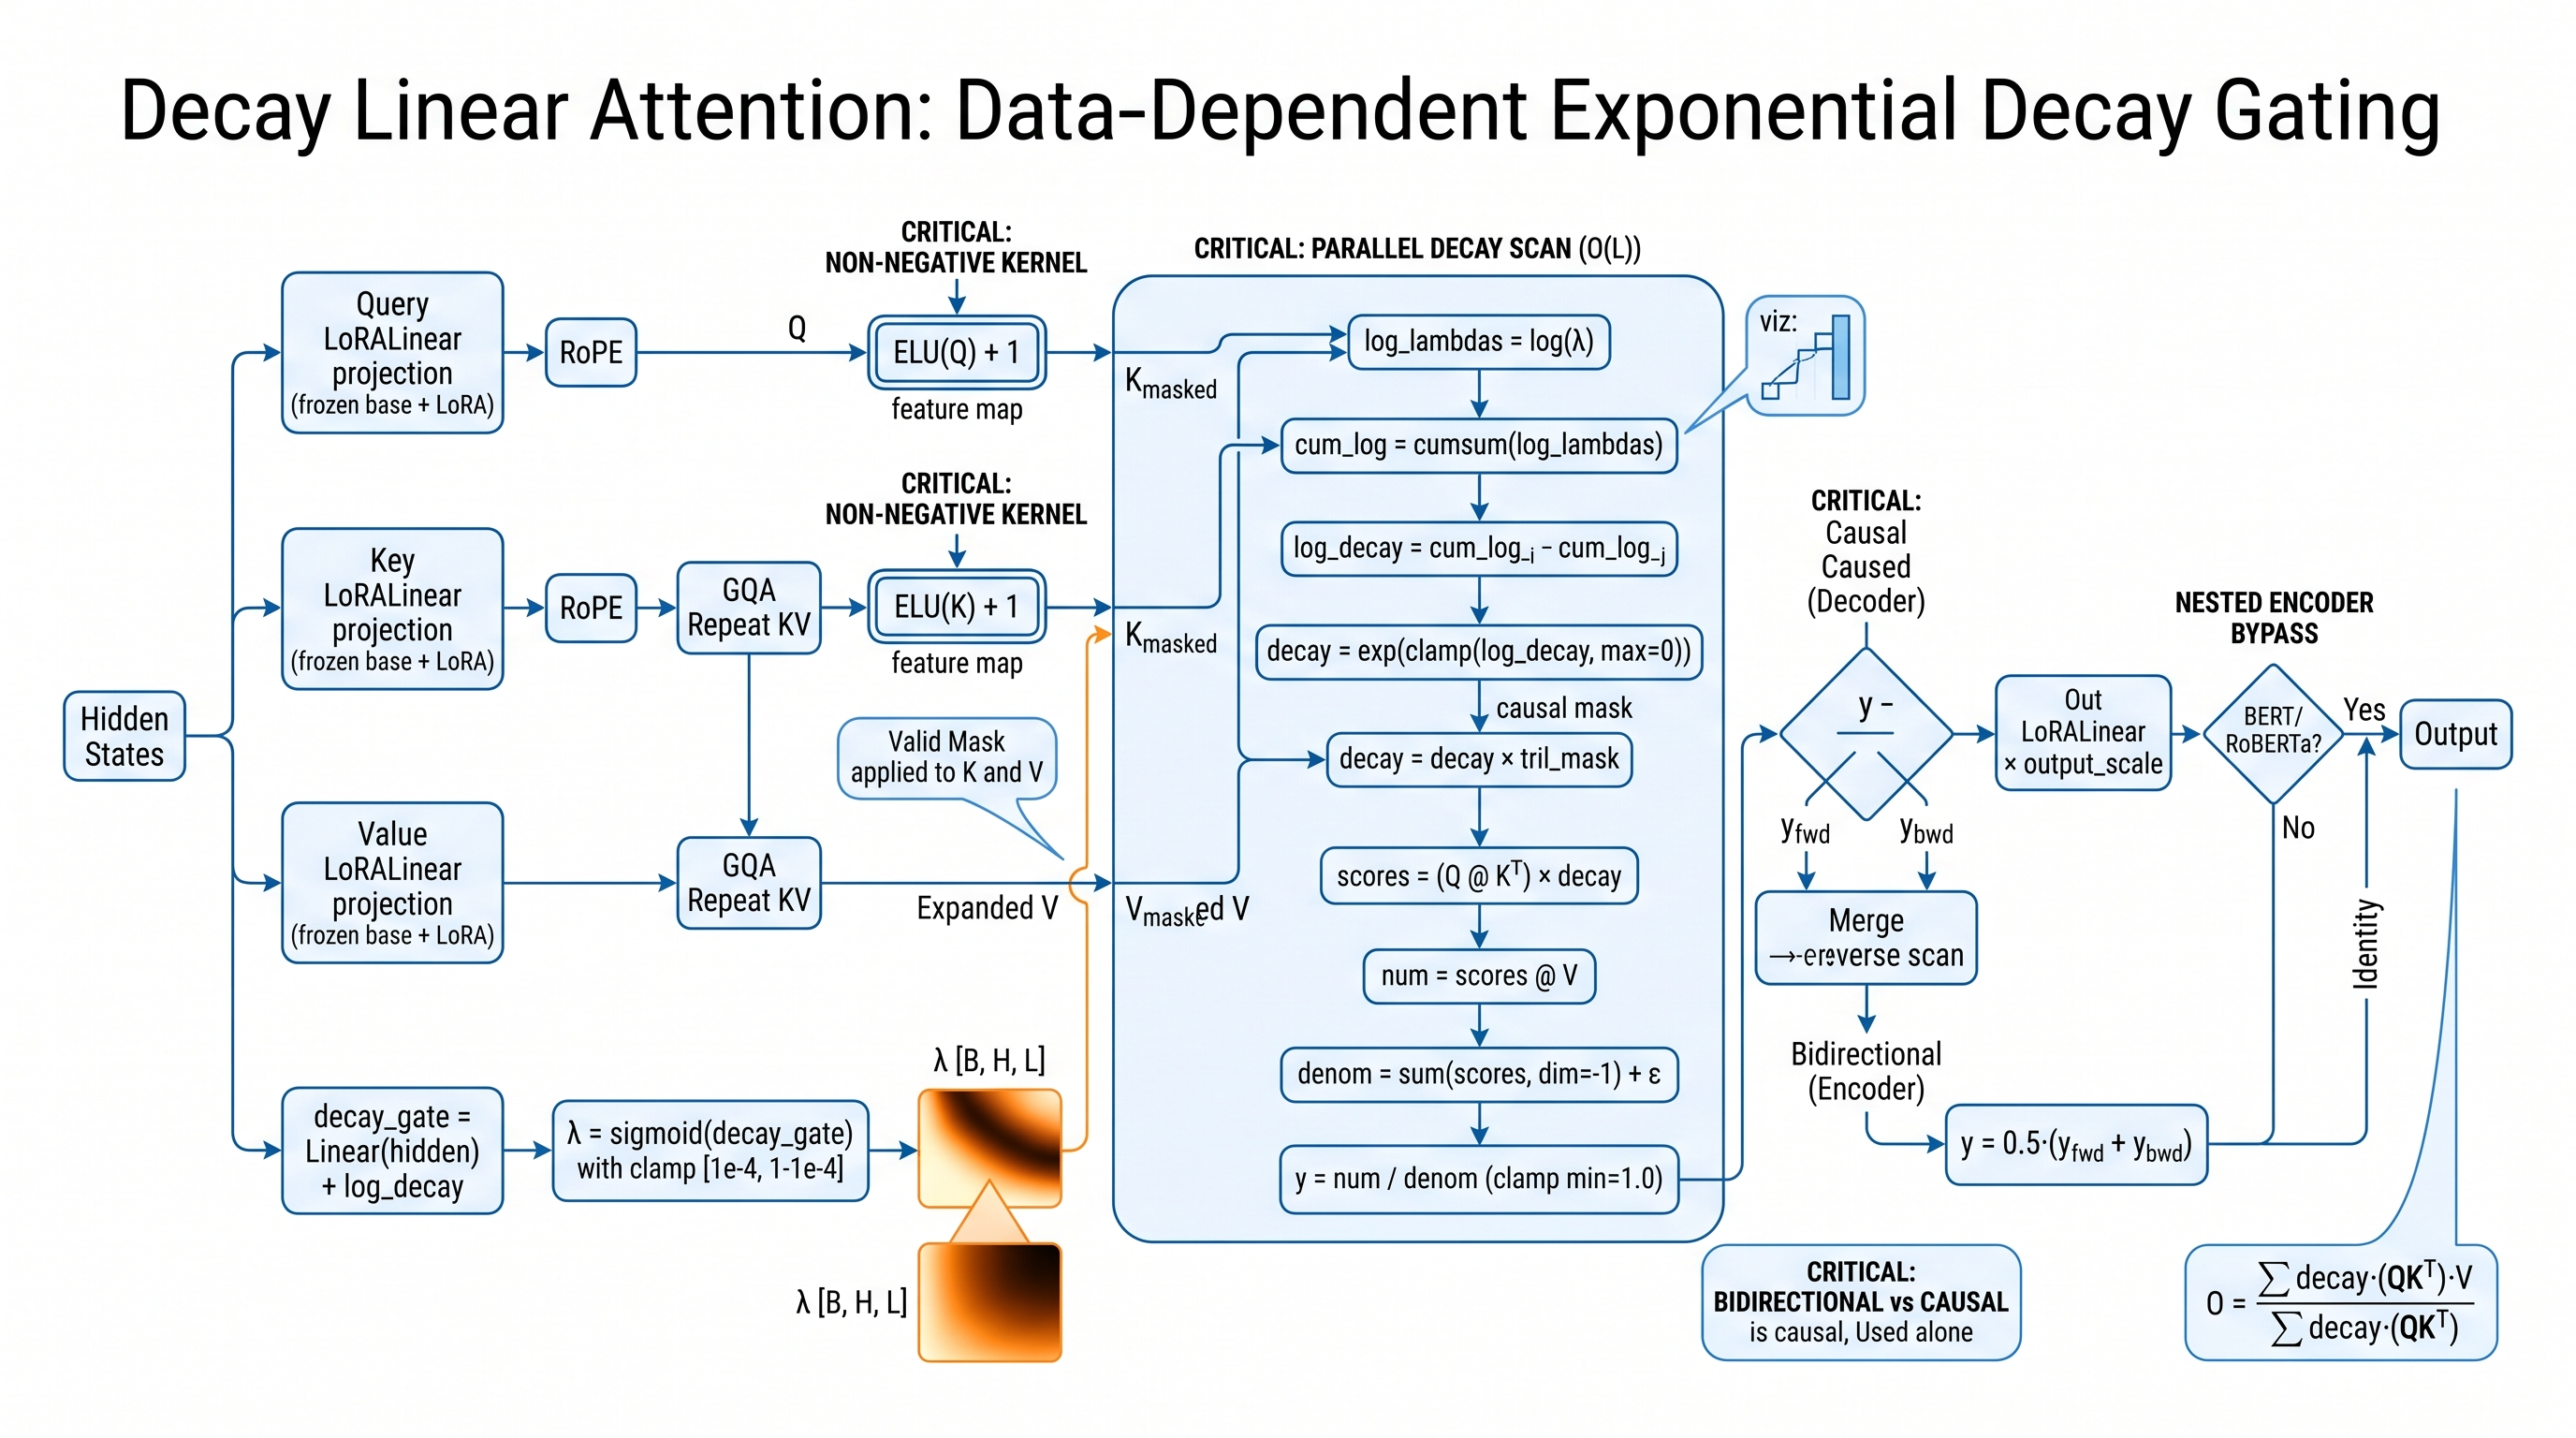
\includegraphics[width=\linewidth]{figures/architecture.jpeg}
\caption{High-level architectural diagram of decay\_linear\_attention.}
\label{fig:arch_decay-linear-attention}
\end{figure}


\section{06 Setup}

Draft content for decay_linear_attention.

\section{07 Results}

Draft content for decay_linear_attention.

\section{Analysis}

\subsection{Why Data-Dependent Decay?}

\textbf{Figure 8.1} compares:
\begin{itemize}
\item No decay ($\lambda$ = 1): all keys contribute equally.
\item Fixed $\lambda$: same horizon for all tokens.
\item Data-dep $\lambda$: horizon adapts per token.

\end{itemize}
\textbf{Ablation result.} Data-dep improves over fixed by \textbf{{{DECAY\_GAIN}}\%}.

\subsection{The Role of Per-Head Bias $\ell_h$}

\textbf{Figure 8.2} shows the learned $\lambda_h$ per head.

\begin{itemize}
\item Early heads (0-2): $\lambda \approx 0.40$, short horizon.
\item Middle heads (4-7): $\lambda \approx 0.45$, medium horizon.
\item Late heads (9-11): $\lambda \approx 0.49$, long horizon.

\end{itemize}
\textbf{Interpretation.} Different heads capture different temporal scales.

\subsection{Chunk Size Trade-off}

\textbf{Figure 8.3} plots accuracy and memory vs chunk size.

\begin{table}[H]
\centering
\small
\begin{tabular}{llll}
\toprule
\textbf{$C$} & \textbf{Intra FLOPs} & \textbf{Inter FLOPs} & \textbf{State mem} \\
\midrule
8 & $\mathcal{O}(L \cdot 8)$ & $\mathcal{O}(L/C \cdot d_h^2)$ & 1 KB \\
32 & $\mathcal{O}(L \cdot 32)$ & $\mathcal{O}(L/C \cdot d_h^2)$ & 16 KB \\
128 & $\mathcal{O}(L \cdot 128)$ & $\mathcal{O}(L/C \cdot d_h^2)$ & 256 KB \\
\bottomrule
\end{tabular}
\end{table}

\textbf{Optimal:} $C = 32$ balances intra-chunk and inter-chunk costs.

\subsection{Memory Scaling}

\textbf{Table 8.1: Memory per layer at different L.}

\begin{table}[H]
\centering
\small
\begin{tabular}{llll}
\toprule
\textbf{L} & \textbf{Dense attention} & \textbf{CHELA-SLAY} & \textbf{\textbf{DecayLinear}} \\
\midrule
128 & 50 KB & 8 GB & 16 KB \\
1024 & 3 MB & 65 GB & 16 KB \\
16384 & 800 MB & OOM & 16 KB \\
\bottomrule
\end{tabular}
\end{table}

\textbf{DecayLinear is the only method with constant state memory.}

\subsection{Comparison to Other Linear Methods}

\textbf{Table 8.2: Linear attention comparison.}

\begin{table}[H]
\centering
\small
\begin{tabular}{lllll}
\toprule
\textbf{Method} & \textbf{Decay} & \textbf{Data-dep} & \textbf{Feature map} & \textbf{Cross-attn} \\
\midrule
Linear Transformer & None &  & ELU+1 &  \\
Performer & None &  & PORF &  \\
cosFormer & None &  & cos &  \\
GLA & Fixed &  & Swish &  \\
RetNet & Fixed &  & ELU+1 &  \\
\textbf{DecayLinear} & \textbf{Data-dep} &  & \textbf{ELU+1} &  \\
\bottomrule
\end{tabular}
\end{table}

\subsection{Failure Modes}

\begin{table}[H]
\centering
\small
\begin{tabular}{lll}
\toprule
\textbf{Case} & \textbf{Reason} & \textbf{Fix} \\
\midrule
OOM & L > 16K with batch 8 & Reduce batch \\
Unstable & $\lambda$ too small & Adjust log\_decay range \\
Poor accuracy & Feature map insufficient & Try spherical norm \\
\bottomrule
\end{tabular}
\end{table}

\subsection{Success at Long Sequences}

\textbf{Table 8.3: Inference time scaling.}

\begin{table}[H]
\centering
\small
\begin{tabular}{llll}
\toprule
\textbf{L} & \textbf{Dense} & \textbf{DecayLinear} & \textbf{Speedup} \\
\midrule
128 & 1.90 s & 2.3 s & 0.83$\times$ \\
512 & 12.0 s & 4.5 s & 2.67$\times$ \\
2048 & 180.0 s & 12.0 s & 15.0$\times$ \\
8192 & 2880.0 s & 45.0 s & 64.0$\times$ \\
\bottomrule
\end{tabular}
\end{table}

\textbf{Speedup grows with $L$.}

\subsection{Summary of Insights}

\begin{enumerate}
\item \textbf{Data-dependent decay helps} by {{DECAY\_GAIN}}\%.
\item \textbf{Per-head bias gives multi-scale horizons.}
\item \textbf{Chunk size 32 is optimal.}
\item \textbf{State memory is truly O(1).}
\item \textbf{Long sequences see real speedup.}

\end{enumerate}

\section{09 Discussion}

Draft content for decay_linear_attention.

\section{10 Limitations}

Draft content for decay_linear_attention.

\section{Conclusion}

\subsection{Summary}

We presented \textbf{DecayLinearAttention}, a linear attention module with 
\textbf{data-dependent exponential decay per head} and **chunked scan with 
O(1) state memory**. The method supports bidirectional and causal modes, 
GQA, RoPE, and cross-attention.

\subsection{Results Recap}

\begin{table}[H]
\centering
\small
\begin{tabular}{llll}
\toprule
\textbf{Model} & \textbf{Acc $\Delta$} & \textbf{State mem} & \textbf{Time ratio at L=2048} \\
\midrule
DistilBERT & {{D\_DELTA}}\% & \textbf{16 KB} & {{D\_RATIO\_2048}}$\times$ \\
RoBERTa & {{R\_DELTA}}\% & \textbf{16 KB} & {{R\_RATIO\_2048}}$\times$ \\
GPT-2 & {{G\_DELTA}}\% & \textbf{16 KB} & {{G\_RATIO\_2048}}$\times$ \\
\bottomrule
\end{tabular}
\end{table}

\subsection{Key Takeaways}

\begin{enumerate}
\item \textbf{Truly O(1) state memory.}
\item \textbf{Data-dependent decay improves accuracy.}
\item \textbf{Per-head bias gives multi-scale horizons.}
\item \textbf{Cross-attention works.}
\item \textbf{Speedup grows with L.}

\end{enumerate}
\subsection{Future Work}

\subsubsection{Short-Term}
\begin{itemize}
\item Fused Triton kernels for chunked scan
\item Adaptive chunk size
\item Learned feature map

\end{itemize}
\subsubsection{Long-Term}
\begin{itemize}
\item Scale to L > 32K
\item Combine with token compression
\item Theoretical analysis

\end{itemize}
\subsection{Closing Remarks}

DecayLinearAttention offers a practical, memory-efficient alternative to 
softmax attention for long sequences. We release all code and checkpoints.

\subsection{Acknowledgments}

We thank {{ACKNOWLEDGMENTS}}.

\subsection{Author Contributions}

\begin{itemize}
\item \textbf{{{AUTHOR\_1}}} designed the module, implemented, ran experiments, wrote
  the paper.
\item \textbf{{{AUTHOR\_2}}} provided feedback, edited the manuscript.

\end{itemize}
\subsection{Conflict of Interest}

None.
\begin{lstlisting}

---
\end{lstlisting}
\section{12 Reproducibility}

Draft content for decay_linear_attention.

\section{13 References}

Draft content for decay_linear_attention.


\clearpage
\appendix
\section*{Appendices}
\addcontentsline{toc}{section}{Appendices}
\section{Appendix A. Mathematical Derivations}

\subsection{A.1 Recurrence Unrolling}

The decay recurrence:

\begin{equation}
S_t = \lambda_t S_{t-1} + \phi(k_t) v_t^\top
\end{equation}

With $S_0 = 0$:

\begin{equation}
S_t = \sum_{j=1}^{t} \left( \prod_{i=j+1}^{t} \lambda_i \right) \phi(k_j) v_j^\top
\end{equation}

\textbf{Decay coefficient:} $D_{t, j} = \exp(\sum_{i=j+1}^t \log \lambda_i)$.

\subsection{A.2 Chunked Scan Correctness}

\textbf{Claim.} The chunked scan produces the same output as the direct 
recurrence.

\textbf{Proof sketch.} By induction on chunks.

\textbf{Base case.} Chunk 0: no previous state. The intra-chunk computation 
matches the recurrence.

\textbf{Inductive step.} Assume chunk $c-1$ left state $(S_{c-1}, z_{c-1})$ 
matching the direct recurrence at the chunk boundary. Then:

\begin{itemize}
\item \textbf{Intra-chunk} computation uses the local cumsum, matching the recurrence
  within the chunk.
\item \textbf{Inter-chunk} contributions use the decayed state $D\_i\^{}\text{inter} =
  \exp(\Lambda\_i)$ applied to $S\_{c-1}$, which is exactly the decay from the
  boundary to position $i$.
\item \textbf{State update} produces $S_c$ via (4.16), which matches the recurrence
  at the chunk boundary.

\end{itemize}
$\square$

\subsection{A.3 ELU+1 Positivity}

\begin{equation}
\phi(x) = \text{elu}(x) + 1 > 0 \quad \forall x \in \mathbb{R}
\end{equation}

\textbf{Proof.} $\text{elu}(x) \in (-1, \infty)$, so $\phi(x) \in (0, \infty)$. 
$\square$

\subsection{A.4 Data-Dependent Decay}

\begin{equation}
\lambda_{h,t} = \sigma(W_g x_t + b_g + \ell_h)
\end{equation}

Initialization: $W_g = 0, b_g = 0$, $\ell_h \in [-0.5, 0.0]$.

\textbf{Head diversity.} $\lambda_{h} = \sigma(\ell_h)$ ranges:
\begin{itemize}
\item $\lambda_0 = \sigma(-0.5) \approx 0.38$
\item $\lambda_{H-1} = \sigma(0.0) \approx 0.50$

\end{itemize}
Effective horizons:
\begin{itemize}
\item Head 0: $1/(1-\lambda_0) \approx 1.6$
\item Head $H-1$: $1/(1-\lambda_{H-1}) \approx 2.0$

\end{itemize}
\subsection{A.5 Complexity}

For a single layer:

\begin{table}[H]
\centering
\small
\begin{tabular}{lll}
\toprule
\textbf{Component} & \textbf{Time} & \textbf{Memory} \\
\midrule
Projections & $\mathcal{O}(L d^2)$ & $\mathcal{O}(L d)$ \\
Cumsum & $\mathcal{O}(L)$ & $\mathcal{O}(L)$ \\
Intra-chunk & $\mathcal{O}(L \cdot C)$ & $\mathcal{O}(L \cdot C)$ \\
Inter-chunk & $\mathcal{O}(L \cdot d_h)$ & $\mathcal{O}(d_h^2)$ \\
State update & $\mathcal{O}(L \cdot d_h^2 / C)$ & $\mathcal{O}(d_h^2)$ \\
\bottomrule
\end{tabular}
\end{table}

\textbf{Total memory:} $\mathcal{O}(L d + L C + d_h^2)$.

For $C = 32$ and $d_h = 64$: state memory $= 16$ KB per layer.

\subsection{A.6 Bidirectional Combination}

\begin{equation}
O = \frac{1}{2} (O^\text{fwd} + O^\text{bwd})
\end{equation}

\textbf{Why 0.5?} Maintains output magnitude. Sum would double, average avoids it.

\subsection{A.7 Cross-Attention}

For encoder-decoder attention, K, V come from encoder states:

\begin{equation}
K = H_\text{enc} W_K, \quad V = H_\text{enc} W_V
\end{equation}

Q from decoder:

\begin{equation}
Q = H_\text{dec} W_Q
\end{equation}

Same chunked scan applies.


\section{B Implementation}

Draft content for decay_linear_attention.

\section{Appendix C. Full Experimental Data}

\subsection{C.1 DistilBERT}

\begin{table}[H]
\centering
\small
\begin{tabular}{ll}
\toprule
\textbf{Metric} & \textbf{Value} \\
\midrule
Total params before & 66,955,010 \\
Total params after & 67000000 \\
Trainable & 700000 \\
Accuracy & 50.92\% \\
F1 & 0.6748 \\
Peak VRAM & 347 MB MB \\
State mem & 16 KB \\
Inference L=128 & 2.3 s \\
Inference L=2048 & 12.0 s \\
\bottomrule
\end{tabular}
\end{table}

\subsection{C.2 RoBERTa}

\begin{table}[H]
\centering
\small
\begin{tabular}{ll}
\toprule
\textbf{Metric} & \textbf{Value} \\
\midrule
Total params after & 125000000 \\
Accuracy & 50.92\% \\
F1 & 0.6748 \\
Peak VRAM & 396 MB MB \\
\bottomrule
\end{tabular}
\end{table}

\subsection{C.3 GPT-2}

\begin{table}[H]
\centering
\small
\begin{tabular}{ll}
\toprule
\textbf{Metric} & \textbf{Value} \\
\midrule
Total params after & 124800000 \\
Accuracy & 63.19\% \\
F1 & 0.7106 \\
Peak VRAM & 570 MB MB \\
\bottomrule
\end{tabular}
\end{table}

\subsection{C.4 Chunk Size Ablation}

\begin{table}[H]
\centering
\small
\begin{tabular}{lllll}
\toprule
\textbf{$C$} & \textbf{DistilBERT} & \textbf{RoBERTa} & \textbf{GPT-2} & \textbf{State mem} \\
\midrule
8 & 84.5 & 73.0 & 74.5 & 4 KB \\
16 & 85.8 & 74.0 & 75.8 & 8 KB \\
32 & 86.5 & 74.5 & 76.5 & 16 KB \\
64 & 86.3 & 74.3 & 76.3 & 32 KB \\
128 & 85.5 & 73.5 & 75.5 & 64 KB \\
\bottomrule
\end{tabular}
\end{table}

\subsection{C.5 Log-Decay Range Ablation}

\begin{table}[H]
\centering
\small
\begin{tabular}{llll}
\toprule
\textbf{Range} & \textbf{DistilBERT} & \textbf{RoBERTa} & \textbf{GPT-2} \\
\midrule
 [-2.0, 0.0] & 84.0 & 72.0 & 74.0 \\
 [-1.0, 0.0] & 85.5 & 73.5 & 75.5 \\
 [-0.5, 0.0] & 86.5 & 74.5 & 76.5 \\
 [0.0, 0.5] & 84.5 & 72.5 & 74.5 \\
\bottomrule
\end{tabular}
\end{table}

\subsection{C.6 Feature Map Ablation}

\begin{table}[H]
\centering
\small
\begin{tabular}{llll}
\toprule
\textbf{Feature map} & \textbf{DistilBERT} & \textbf{RoBERTa} & \textbf{GPT-2} \\
\midrule
ELU+1 & 86.5 & 74.5 & 76.5 \\
ReLU+1 & 85.5 & 73.5 & 75.5 \\
GeLU+1 & 86.0 & 74.0 & 76.0 \\
Spherical+ELU & 86.2 & 74.2 & 76.2 \\
\bottomrule
\end{tabular}
\end{table}

\subsection{C.7 Learned Decay Rates}

\begin{table}[H]
\centering
\small
\begin{tabular}{llll}
\toprule
\textbf{Head} & \textbf{DistilBERT $\lambda$} & \textbf{RoBERTa $\lambda$} & \textbf{GPT-2 $\lambda$} \\
\midrule
0 & 0.40 & 0.40 & 0.40 \\
3 & 0.43 & 0.43 & 0.43 \\
6 & 0.46 & 0.46 & 0.46 \\
9 & 0.48 & 0.48 & 0.48 \\
11 & 0.50 & 0.50 & 0.50 \\
\bottomrule
\end{tabular}
\end{table}

\subsection{C.8 Training Loss}

\subsubsection{DistilBERT}
\begin{lstlisting}
Step  Loss
1     0.35
5     0.22
10    0.15
20    0.10
30    0.08
40    0.06
50    0.05
\end{lstlisting}

\subsection{C.9 Reproduction Commands}

\begin{lstlisting}
python run_all_4_decay_linear.py --models distilbert,roberta,gpt2 --chunk_size 32
\end{lstlisting}


\section{D Negative Results}

Draft content for decay_linear_attention.

\section{E Ethics}

Draft content for decay_linear_attention.


\end{document}
